\documentclass{beamer}
\usetheme{metropolis}
%\setbeamersize{text margin left=.2cm,text margin right=.2cm}
\usepackage{graphicx}
\graphicspath{{../../images/}}
%\usepackage[french]{babel}
%\usepackage{listings}
%\usepackage{lipsum}
\usepackage{boolexpr}
\usepackage{kpfonts}
\usepackage{caption}
\usepackage{wrapfig}
\usepackage{tkz-graph}
\usepackage{tikz}
%\usepackage{chngcntr}
\usepackage[labelformat=empty]{caption}
\usepackage[official]{eurosym}

\usepackage{minted}

\usepackage{siunitx}

% http://tex.stackexchange.com/questions/114830/how-can-i-use-lvert-and-rvert-norm-symbols-x-with-the-iwona-math-font
\usepackage[math]{iwona}
\usepackage{scalerel}
\def\lVert{\mid\!\mid}
\def\rVert{\mid\!\mid}

\usepackage[normalem]{ulem}
%\newcommand{\Adj}{\mathbf{A}}
\usepackage{mathtools}

\usepackage{../../custom}
\usepackage{amsfonts}
%\newcommand{\jsrcodepath}{../../code}
%\usepackage{jsr}

\newcommand{\expe}[2]{\la #1, #2 \ra}

\usepackage{framed}

%\usepackage{mathtools,xparse}
%\DeclarePairedDelimiter{\norm}{\lVert}{\rVert}
\newcommand\Wider[2][3em]{%
\makebox[\linewidth][c]{%
  \begin{minipage}{\dimexpr\textwidth+#1\relax}
  \raggedright#2
  \end{minipage}%
  }%
}

\newcommand{\aeur}{\alpha_\text{\euro}}
\newcommand{\adol}{\alpha_\$}
\newcommand{\apou}{\alpha_\text{\pounds}}

\title{Polynomial and Moment Optimization in Julia and JuMP}
\date{August 24, 2019}
\author{Tillmann Weisser (LANL), Beno\^it Legat (UCLouvain), Chris Coey (MIT), Lea Kapelevich (MIT), Juan Pablo Vielma (MIT)}
%\institute{Los Alamos National Laboratory, 16th July 2019}
%\institute{UCLouvain\\
%           Massachusetts Institute of Technology (MIT)\\
%           Rice University\\
%           Los Alamos National Laboratory (LANL)}

% https://tex.stackexchange.com/questions/426088/texlive-pretest-2018-beamer-and-subfig-collide
\makeatletter
\let\@@magyar@captionfix\relax
\makeatother
\begin{document}
  \maketitle

\begin{frame}
  \frametitle{Polynomial Optimization community}
  \begin{itemize}
    \item Subcommunity of JuMP-dev community.
    \item Gitter channel: \url{https://gitter.im/JuliaOpt/SumOfSquares.jl}.
    \item Optimization packages: SumOfSquares, PolyJuMP, MomentOpt, Hypatia
    \item Depends on JuliaAlgebra packages: MultivariatePolynomials (implementations: DynamicPolynomials, TypedPolynomials),
      SemialgebraicSets, MultivariateBases, MultivariateMoments.
    \item Fast growing community (alphabetical order):
      Paul Breiding,
      Robin Deits,
      Marcelo
      Forets,
      Joey Huchette,
      Bernard Mourrain,
      Amelia Perry,
      Sascha Timme...
    \item JuMP GSOC projects benefits polynomial optimization:
      Arpit Bhatia (examples),
      Guilherme Bodin (Automatic Dualization) and
      Gilles Peiffer (Mutable Arithmetics).
  \end{itemize}
\end{frame}

\begin{frame}{Overview}
\Wider[4em]{
  \begin{center}
    \begin{tikzpicture}[scale=0.9]
      \draw[rounded corners=5pt, fill=aurore!70] (-1.8, 3.5) rectangle (1.8, 4.5);
      \node at (0, 4) {\jlpkg{MomentOpt}};
      \draw[rounded corners=5pt, fill=frambo!50] (-2, 1.5) rectangle (2, 2.5);
      \node at (0, 2) {\jlpkg{SumOfSquares}};
      \node at (0, 0) {
\includegraphics[scale=0.2]{JuMP.png}};
      \draw[->, line width=1pt] (0, 3.5) to (0, 2.5);
      \draw[->, line width=1pt] (0, 1.5) to (0, 0.3);
      %\draw[rounded corners=5pt] (-3, -6.5) rectangle (3, -1.5);
      %\node[rotate=90] at (-2.7, -4) {\jlpkg{MathOptInterface}};
      %\node[rotate=-90] at (2.7, -4) {MOI};
      \draw[rounded corners=5pt, fill=lichen!70] (0.8, -2.5) rectangle (3.2, -1.5);
      \node at (2, -2) {SOSBridge};
      %\draw[rounded corners=5pt, fill=aurore!70] (-1, -4.5) rectangle (1, -5.5);
      %\node at (0, -5) {Caching};
      %\draw[->, line width=1pt] (0, -3.5) to (0, -4.5);
      \draw[->, line width=1pt] (-0.5, -0.8) to (-3, -3.5);
      \draw[->, line width=1pt] (0.5, -0.8) to (0.9, -1.5);
      \draw[->, line width=1pt] (3, -2.5) to (3.5, -3.5);
      \draw[rounded corners=5pt, fill=canard!60] (-5.2, -4.5) rectangle (-2.8, -3.5);
      \node at (-4, -4) {\jlpkg{Hypatia}};
      \draw[rounded corners=5pt, fill=canard!60] (2.5, -4.5) rectangle (5.5, -3.5);
      \node at (4, -4) {SDP solver};
    \end{tikzpicture}
  \end{center}
}
\end{frame}

  \begin{frame}
    \tableofcontents
  \end{frame}

\section{MathOptInterface Bridges}

  \begin{frame}[fragile]
    \frametitle{MathOptInterface (MOI)}
    MOI in a nutshell:
    \begin{itemize}
      \item \verb|add_variable(model)|, \verb|add_constrained_variable(model, set)|.
      \item \verb|add_constraint(model, func, set)|, e.g. $2x + 3y = 1$ $\to$ (\verb|2*x + 3*y|)-in-\verb|EqualTo(1.0)|.
      \item \verb|set|, \verb|get| attributes, e.g., \verb|ObjectiveFunction|.
    \end{itemize}
    Extensible framework:
    \begin{itemize}
      \item \alert{Generic} on attribute, function and set types. New ones can be defined \alert{independently}.
      \item Solver-\alert{specific} features easily exposed to JuMP/MOI users through \alert{custom} attributes.
      \item Expose \alert{specialized} problem structure easily through \alert{custom} functions, sets (e.g. Sum-of-Squares variables/constraints).
    \end{itemize}
  \end{frame}

  \begin{frame}{Semidefinite programming}
    \begin{align*}
      \mini_{Q \in \SymK} \quad & \la C, Q \ra & \maxi_{y \in \R^n} \quad & \la b, y \ra\\
      \subtoq & \la A_i, Q \ra = b_i & \subtoq & \sum_i A_i y_i \preceq C\\
        & Q \succeq 0
    \end{align*}
    \textbf{File format}: SDPA

    \textbf{Solvers}: CSDP, SDPA, DSDP, SDPLR, ...

    \textbf{Variables}: $Q$ block diagonal, nonnegative scalar variables ($1 \times 1$ blocks) or SDP matrices.

    \textbf{Constraints}: Affine equations.
  \end{frame}

  \begin{frame}[fragile]
    \frametitle{Conic Modelling}
\begin{minted}{Julia}
using JuMP
model = Model(...)
@variable(model, -1 <= x <= 1)
@variable(model, y)
@variable(model, z <= 0)
@constraint(model, [x + y x
                    y     x - y] in PSDCone())
@constraint(model, [x + y, z, y] in SecondOrderCone())
@objective(model, x^2 - 2x*z + z^2)
\end{minted}
  \end{frame}

  \begin{frame}
    \frametitle{The gap between models and solvers}
    The solver interface should only support structures and the algorithm \alert{exploits}:
    \begin{itemize}
      \item
        $n$ solvers and $m$ structures $\to$ $mn$ transformations $\to$ \alert{unscalable} for large $m, n$.
      \item
        enables \alert{evaluation} of formulation \alert{quality}, e.g. automatic transformation and
        automatic dualization.
    \end{itemize}

    The model should
    \begin{itemize}
      \item be \alert{independent} from solvers.
      \item represent the structure \alert{exploitable} by algorithms.
      \item allow reprentable structure \alert{unknown} to solvers, e.g. Sum-of-Squares variables/constraints.
    \end{itemize}
  \end{frame}

%\section{Examples}

  \begin{frame}[allowframebreaks]
    \frametitle{Examples}
    \begin{block}{FlipSignBridge}
      \begin{itemize}
        \item \textbf{Variable} $x \ge l$ substituted by $x = -y$ where $y \le -l$.
        \item \textbf{Constraint} $a^\top x \le \beta$ transformed into $-a^\top x \ge -\beta$.
      \end{itemize}
    \end{block}
    \begin{block}{VectorizeBridge}
      \begin{itemize}
        \item \textbf{Variable} $x \ge l$ substituted by $x = y + l$ where $y \in \R^1_+$.
        \item \textbf{Constraint} $a^\top x \le \beta$ transformed into $[a^\top x - \beta] \in \R^1_-$.
      \end{itemize}
    \end{block}
    \begin{block}{IntervalBridge}
      \begin{itemize}
        \item \textbf{Constraint} $l \le a^\top x \le u$ transformed into $a^\top x \ge l$ and $a^\top x \le u$.
      \end{itemize}
    \end{block}
    \begin{block}{IndicatorBridge}
      \begin{itemize}
        \item \textbf{Constraint} $y$ binary, $\neg y \Rightarrow a^\top x \le \beta$ transformed into $z$ binary, $z + y = 1$ and $z \Rightarrow a^\top x \le \beta$.
      \end{itemize}
    \end{block}
%    \begin{block}{ZerosBridge}
%      \begin{itemize}
%        \item \textbf{Variable} $x \in \{\mathbf{0}_n\}$ transformée en $x = \mathbf{0}_{n \times 0}y$ pour $y \in \R^0$.
%      \end{itemize}
%    \end{block}
    \begin{block}{FreeBridge}
      \begin{itemize}
        \item \textbf{Variable} $x \in \R$ substituted by $x = y + z$ where $y \in \R_+$ and $z \in \R_-$.
      \end{itemize}
    \end{block}

    \begin{block}{SlackBridge}
      \begin{itemize}
        \item \textbf{Constraint} $f \in S$ transformed into $f = x$ for variable $x \in S$.
        \item \textbf{Objective} $\min f$ transformed into $\min x$ with $f \le x$.
      \end{itemize}
    \end{block}
  \end{frame}

%\section{Combining bridges}

\begin{frame}{Interval constraint for SDPA}
\Wider[4em]{
  \begin{center}
    \begin{tikzpicture}[xscale=4.5, yscale=2]
      \tikzset{VertexStyle/.style = {}}
      \Vertex[x=1, y=-1, L={$a^\top x + \beta \ge l$}]{G}
      \Vertex[x=2, y=-1, L={$a^\top x + \beta \le u$}]{L}
      \Vertex[x=1, y=-2, L={$A x + b \in \mathbb{R}_+^1$}]{N}
      \Vertex[x=2, y=-2, L={$A x + b \in \mathbb{R}_-^1$}]{P}
      \Vertex[x=1, y=-3, L={$A x + b \in \{0\}^1$}]{Z}
      \Vertex[x=0, y=0, L={$x \le u$}]{VL}
      \Vertex[x=0, y=-1, L={$x \ge l$}]{VG}
      \Vertex[x=0, y=-2, L={$x \in \mathbb{R}_-^1$}]{VP}
      \tikzset{VertexStyle/.style = {
        shape = rectangle,
        draw
      }}
      \Vertex[x=1, y=0, L={$l \le a^\top x + \beta \le u$}]{I}
      \tikzset{VertexStyle/.style = {
        shape = rounded rectangle,
        draw
      }}
      \Vertex[x=2, y=-3, L={$a^\top x = \beta$}]{E}
      \Vertex[x=0, y=-3, L={$x \in \mathbb{R}_+^1$}]{VN}
      \tikzset{EdgeStyle/.style = {->}}
      \Edge[label={flip}](L)(G)
      \Edge[label={flip}](VP)(VN)
      \Edge[label={flip}](VL)(VG)
      \Edge[label={split}](I)(L)
      \Edge[label={split}](I)(G)
      \Edge[label={vectorize}](G)(N)
      \Edge[label={vectorize}](L)(P)
      \Edge[label={scalarize}](Z)(E)
      \Edge[label={slack}](P)(Z)
      \Edge[label={slack}](N)(Z)
      \Edge[label={slack}](N)(VN)
      \Edge[label={slack}](G)(VG)
      \tikzset{EdgeStyle/.style = {->, pos=0.3}}
      \Edge[label={slack}](G)(E)
      \tikzset{EdgeStyle/.style = {->, bend left=22, pos=0.3}}
      \Edge[label={slack}](P)(VP)
      \tikzset{EdgeStyle/.style = {->, bend left=20, pos=0.7}}
      \Edge[label={vectorize}](VL)(VP)
      \tikzset{EdgeStyle/.style = {->, bend left=25, pos=0.8}}
      \Edge[label={slack}](L)(E)
      \tikzset{EdgeStyle/.style = {->, bend right=20, pos=0.3}}
      \Edge[label={vectorize}](VG)(VN)
      \tikzset{EdgeStyle/.style = {->, bend right=25}}
      \tikzset{EdgeStyle/.style = {->, bend right=60, pos=0.2}}
      \Edge[label={slack}](L)(VL)
      \tikzset{EdgeStyle/.style = {->}}
      \Edge[label={flip}](P)(N)
    \end{tikzpicture}
  \end{center}
}
\end{frame}

%\section{Automatic selection of bridges}

%\begin{frame}
%  \frametitle{Selection of bridges}
%  How to select bridges \alert{automatically} ?
%
%  \begin{block}{Example}
%    Free variable for SDP solver:
%    \begin{itemize}
%      \item FreeBridge: $x \in \R$ $\to$ $y \in \R_+$ (supported) and $z \in \R_-$ (\alert{not} supported)
%      \item FlipSignBridge: $x \in \R_-$ $\to$ $y \in \R_+$.
%    \end{itemize}
%  \end{block}
%
%  Shortest path ?
%\end{frame}

\begin{frame}
  \frametitle{Bridges directed hypergraph}
  \vspace{-.2cm}
  \begin{block}{Nodes}
    Node for each set $S$ (variable-in-$S$).

    Node for each constraint $F$-in-$S$.

    Node for each objective function $F$.

    %Types $F$ and $S$ are \alert{not limited} to those defined in MOI.

    %\alert{Infinitely} many nodes, we need to be \alert{lazy}.
  \end{block}
  \vspace{-.2cm}
  \begin{block}{Edges}
    %Each bridge defined possible \alert{infinitely} many edges.

    For each edge and ingoing node: outgoing nodes are
    \begin{itemize}
        \item variable-in-$S$ created.
        \item constraints $F$-in-$S$ created.
        \item objective $F$ set.
    \end{itemize}
  \end{block}
  %\vspace{-.2cm}

  %Solved by a modified \alert{Bellman-Ford} algorithm.
\end{frame}

\begin{frame}
  \frametitle{Bridges selection}

  \begin{block}{Multiple dispatch ?}
    Can we use multiple dispatch where node types are method signatures ?

    \textbf{No}.
    Several bridge can transform same types.
    Dispatching on more specialized is not accurate.

    Need to guide choice to supported types.
  \end{block}

  \begin{block}{Just in Time (JIT) bridge selection}
    Types $F$ and $S$ are \alert{not limited} to those defined in MOI $\to$
    \alert{infinitely} many nodes.

    Each bridge defined possible \alert{infinitely} many edges.

    Need to be \alert{lazy} and compute bridge selection JIT when
    type first used.
  \end{block}

\end{frame}

\begin{frame}
  \frametitle{Bridge selection algorithm}
  \textbf{Data}: Set of bridges $B$

  \textbf{Invariant}: $d_\mathcal{V}$, $d_\mathcal{C}$, $d_\mathcal{O}$
  are correct when defined.

  Given new type: compute types $T$ where $d$ should be defined with
  Depth First Search (DFS) from the type: $\mathcal{O}(|B|)$.

  Compute $d$ at the types using Bellman-Ford algorithm: $\mathcal{O}(|T| \cdot |B|)$.
\end{frame}

\section{Extending JuMP}

\begin{frame}[fragile]
  \frametitle{Extending JuMP macros}
\begin{minted}{Julia}
@constraint(model, [x + 1, x - y] in MOI.Zeros())
\end{minted}
  Implementation:
\begin{minted}{Julia}
function build_constraint(
    _error::Function,
    func::Vector, set::MOI.AbstractVectorSet)
    return VectorConstraint(x, set)
end
function add_constraint(model, c::AbstractConstraint,
                        name)
    index = MOI.add_constraint(backend(model),
        moi_function(c), moi_set(c))
    ... # set name and shape
    return ConstraintRef(model, index, shape(c))
end
\end{minted}
\end{frame}

\begin{frame}[fragile]
  \frametitle{Extending JuMP macros: Custom set}
\begin{minted}{Julia}
@constraint(model, [x + 1, x - y] in SecondOrderCone())
\end{minted}
  Implementation:
\begin{minted}{Julia}
function build_constraint(_error::Function,
                          f::AbstractVector,
                          s::AbstractVectorSet)
    set = moi_set(s, length(f))
    return build_constraint(_error, f, set)
end
function moi_set(::SecondOrderCone, dim::Int)
  return MOI.SecondOrderCone(dim)
end
\end{minted}
\end{frame}

\begin{frame}[fragile]
  \frametitle{Extending JuMP macros: PSD cone}
\begin{minted}{Julia}
using LinearAlgebra # For Symmetric
@constraint(model, Symmetric([x + 1 x - y
                              x - y y]) in PSDCone())
\end{minted}
  Implementation:
\begin{minted}{Julia}
function build_constraint(_error::Function,
                          Q::Symmetric,
                          ::PSDCone)
    n = LinearAlgebra.checksquare(Q)
    func = [Q[i, j] for j in 1:n for i in 1:j]
    set = MOI.PositiveSemidefiniteConeTriangle(n)
    VectorConstraint(func, set,
                     SymmetricMatrixShape(n))
end
\end{minted}
\end{frame}

\begin{frame}[fragile]
  \frametitle{Adding bridges}
\begin{minted}{Julia}
struct BridgeableConstraint{C, B} <: AbstractConstraint
    constraint::C
    bridge_type::B
end

function add_constraint(model::Model,
                        c::BridgeableConstraint,
                        name::String="")
    add_bridge(model, c.bridge_type)
    return add_constraint(model, c.constraint, name)
end
\end{minted}
\end{frame}

\section{Sum-of-Squares extension}

  \begin{frame}{Nonnegative quadratic forms into sum of squares}
    \begin{tikzpicture}
      \draw[->, bend left=30] (-1, 1.6) node[left] {$(x_1, x_2, x_3)$} to (-.1, 1.3);
      \draw[->, bend left=30] (-1, 1.6) to (.9, 1.25);
      \draw[->, bend right=30] (2.1, 2) node[right] {\alert{unique}} to (1.55, 1.35);
      \node at (-.2, 1.2) {$p(x)$};
      \node at (.5, 1.2) {$=$};
      \node at (1.3, 1.2) {$x^\Tr Q x$};
      \node at (-2.4, 0) {$x_1^2 + 2x_1x_2 + 5x_2^2 + 4x_2x_3 + x_3^2$};
      \node at (.5, 0) {$=$};
      \node at (2.4, 0) {$x^\Tr \begin{pmatrix}1 & 1 & 0\\1 & 5 & 2\\ 0 & 2 & 1\end{pmatrix} x$};
      \node at (-1, -1.5) {$p(x) \geq 0$ $\forall x$};
      \node at (1.5, -1.5) {$Q \succeq 0$};
      \node at (.5, -1.5) {$\Longleftrightarrow$};
      \draw[->] (2.5, -1) to node[right] {cholesky} (2.5, -2.5);
      \node at (-3, -3.5) {$(x_1 + x_2)^2 + (2x_2 + x_3)^2$};
      \draw[->] (.2, -3.5) to (-.8, -3.5);
      \node at (3, -3.5) {$x^\Tr \begin{pmatrix}1 & 1 & 0\\0 & 2 & 1\end{pmatrix}^\Tr \begin{pmatrix}1 & 1 & 0\\0 & 2 & 1\end{pmatrix} x$};
    \end{tikzpicture}
  \end{frame}

  \begin{frame}{Nonnegative polynomial into sum of squares}
    \begin{tikzpicture}
      \draw[->, bend left=30] (-1, 1.6) node[left] {$(x_1, x_2, x_3)$} to (-.1, 1.3);
      \draw[->, bend left=20] (.6, 1.6) node[above] {$(x_1, x_1x_2, x_2)$} to (.9, 1.35);
      \draw[->, bend right=30] (2.1, 2) node[right] {\alert{\emph{not} unique}} to (1.55, 1.35);
      \node at (-.1, 1.2) {$p(x)$};
      \node at (.5, 1.2) {$=$};
      \node at (1.3, 1.2) {$X^\Tr Q X$};
      \node at (-2.5, 0) {$x_1^2 + 2x_1^2x_2 + 5x_1^2x_2^2 + 4x_1x_2^2 + x_2^2$};
      \node at (.5, 0) {$=$};
      \node at (2.3, 0) {$X^\Tr \begin{pmatrix}1 & 1 & 0\\1 & 5 & 2\\ 0 & 2 & 1\end{pmatrix} X$};
      \node at (-1, -1.5) {$p(x) \geq 0$ $\forall x$};
      \node at (1.5, -1.5) {$Q \succeq 0$};
      \node at (.5, -1.5) {$\Longleftarrow$};
      \draw[->] (2.5, -1) to node[right] {cholesky} (2.5, -2.5);
      \node at (-3, -3.5) {$(x_1 + x_1x_2)^2 + (2x_1x_2 + x_2)^2$};
      \draw[->] (.2, -3.5) to (-.6, -3.5);
      \node at (3, -3.5) {$X^\Tr \begin{pmatrix}1 & 1 & 0\\0 & 2 & 1\end{pmatrix}^\Tr \begin{pmatrix}1 & 1 & 0\\0 & 2 & 1\end{pmatrix} X$};
    \end{tikzpicture}
  \end{frame}

  \begin{frame}{When is nonnegativity equivalent to sum of squares ?}
    Determining whether a polynomial is nonnegative is \alert{NP-hard}.
    \begin{block}{Hilbert 1888}
      Nonnegativity of $p(x)$ of $n$ variables and degree $2d$ is equivalent to sum of squares in the following three cases:
      \begin{itemize}
        \item $n = 1$ : Univariate polynomials
        \item $2d = 2$ : Quadratic polynomials
        \item $n = 2$, $2d = 4$ : Bivariate quartics
      \end{itemize}
    \end{block}
    \begin{columns}
      \begin{column}{0.7\textwidth}
    \begin{block}{Motzkin 1967}
      First \alert{explicit} example:
      \[ x_1^4x_2^2 + x_1^2x_2^4 + 1 - 3x_1^2x_2^2 \geq 0 \quad \forall x \]
      but is \alert{not} a sum of squares.
    \end{block}
      \end{column}
      \begin{column}{0.3\textwidth}
        \centering
        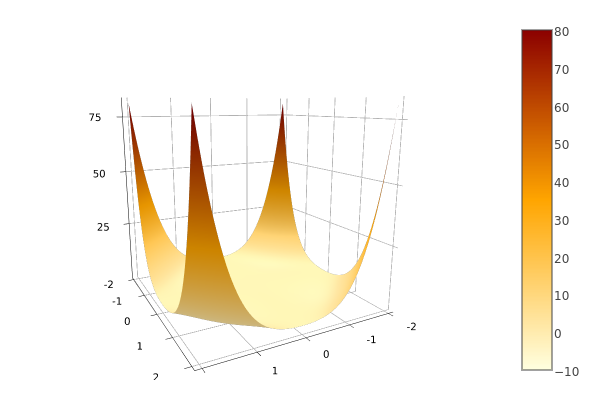
\includegraphics[trim=3cm .7cm 6cm 3cm, clip, width=\textwidth]{motzkin.png}
      \end{column}
    \end{columns}
  \end{frame}

  \begin{frame}
    \frametitle{Theory behind bridges}
    \[ x \in S_1 \Leftrightarrow Ax \in S_2 \qquad AS_1 = S_2 \]
    \[ A^* y \in S_1^* \Leftrightarrow y \in S_2^* \qquad S_1^* = A^* S_2^* \]
    In Lagrangian:
    \[ \langle Ax, y \rangle_2 = \langle x, A^* y \rangle_1 \]
    \vspace{-0.5cm}
    \begin{block}{Transformation of variable-in-$S_2$ to variable-in-$S_1$.}
%      \[ Ax \in S_1 \Leftrightarrow x \in S_2 \qquad S_1 = AS_2 \]
%      \[ y \in S_1^* \Leftrightarrow A^* y \in S_2^* \qquad A^* S_1^* = S_2^* \]
%
%      Dans un Lagrangien:
%      \[ \langle x, A^* y \rangle_2 = \langle A x, y \rangle_1 \]
      \begin{enumerate}
        \item[Primal] Transform value $v$ to $Av$.
        \item[Dual] Transform dual $y$ to $A^{-*}y$.
      \end{enumerate}
    \end{block}
    \begin{block}{Transformation of $f$-in-$S_1$ constraint to $Af$-in-$S_2$ constraint.}
      %Transforme constraint $f$-in-$S_1$ en $Af$-in-$S_2$.

      \begin{enumerate}
        \item[Primal] Transform value $v$ of $Af$ to $A^{-1}v$ of $f$.
        \item[Dual] Transform dual $y$ of $A^*y$.
      \end{enumerate}
    \end{block}
  \end{frame}

\begin{frame}
  \frametitle{Sum-of-Squares bridges}
  Polynomial $p \in \Sigma$ ($p$ is SOS) iff
  $p = X^\top Q x$ with $Q \in \mathbb{S}_+$ ($Q$ is PSD).
  Hence $\Sigma = A \mathbb{S}_+$.

  SOSPolnomialBridge: Transformation of variable-in-$\Sigma$ to variable-in-$\mathbb{S}_+$.

  Transformation of contraint $F$-in-$\Sigma$: SlackBridge + SOSPolnomialBridge.
\end{frame}

\begin{frame}
  \frametitle{Result transformations}
  \begin{block}{Constraint Attribute}
    \textbf{Examples}: ConstraintPrimal, ConstraintDual, ConstraintFunction, ConstraintSet, ...

    \alert{Redirected} to bridge when constraint is bridged.
  \end{block}
  New attributes:
  \begin{itemize}
    \item GramMatrixAttribute: Gram matrix $Q$ indexed by $X$.
    \item MomentMatrixAttribute: Moment matrix index by $X$, dual of constraint $Q \in \mathbb{S}_+$.
    \item MomentsAttribute: Vector of moments, dual of constraint $p = X^\top Q X$.
  \end{itemize}
\end{frame}

\begin{frame}[fragile]
  \frametitle{Sum-of-Squares constraint macro}
\begin{minted}{Julia}
@constraint(model, p in SOSCone())
\end{minted}
  Implementation:
\begin{minted}{Julia}
function JuMP.build_constraint(_error::Function, p,
                               cone::SOSCone; kws...)
    coefs = coefficients(p)
    monos = monomials(p)
    set = JuMP.moi_set(cone, monos; kws...)
    shape = PolyJuMP.PolynomialShape(monos)
    return PolyJuMP.bridgeable(
        JuMP.VectorConstraint(coefs, set, shape),
        JuMP.moi_function_type(typeof(coefs)),
        typeof(set)
    )
end
\end{minted}
\end{frame}

\section{Reshaping}

\begin{frame}[fragile]
  \frametitle{Reshaping sets}
\begin{minted}{Julia}
function reshape_set(set::MOI.AbstractScalarSet,
                     ::ScalarShape)
    return set
end
function reshape_set(
    ::MOI.PositiveSemidefiniteConeTriangle,
    ::SymmetricMatrixShape
)
    return PSDCone()
end
\end{minted}
\end{frame}

\begin{frame}[fragile]
  \frametitle{Reshaping polynomial sets}
\begin{minted}{Julia}
function JuMP.reshape_set(set::SOSPolynomialSet,
                          ::PolyJuMP.PolynomialShape)
    return set.cone
end
\end{minted}
\end{frame}

\begin{frame}[fragile]
  \frametitle{Reshaping results}
\begin{minted}{Julia}
function reshape_vector(vectorized_form::Vector{T},
        shape::SymmetricMatrixShape) where T
    matrix = Matrix{T}(undef, shape.side_dimension,
                       shape.side_dimension)
    k = 0
    for j in 1:shape.side_dimension
        for i in 1:j
            k += 1
            matrix[j, i] = matrix[i, j] =
                vectorized_form[k]
        end
    end
    return Symmetric(matrix)
end
\end{minted}
\end{frame}

\begin{frame}[fragile]
  \frametitle{Reshaping polynomial results}
\begin{minted}{Julia}
function JuMP.reshape_set(set::SOSPolynomialSet,
                          ::PolyJuMP.PolynomialShape)
    return set.cone
end
function JuMP.reshape_vector(x::Vector,
                             shape::PolynomialShape)
    return polynomial(x, shape.monomials)
end
function JuMP.reshape_vector(x::Vector,
                             shape::MomentsShape)
    return measure(x, shape.monomials)
end
\end{minted}
\end{frame}

\begin{frame}[fragile]
  \frametitle{Dual shape}
  In JuMP:
\begin{minted}{Julia}
dual_shape(shape::AbstractShape) = shape
\end{minted}
  In PolyJuMP:
\begin{minted}{Julia}
function JuMP.dual_shape(shape::PolynomialShape)
    return MomentsShape(shape.monomials)
end
function JuMP.dual_shape(shape::MomentsShape)
    return PolynomialShape(shape.monomials)
end
\end{minted}
\end{frame}

\end{document}
